\paragraph{}
Our timeline (Figure~\ref{fig:project_timeline}), named \textit{Muirhead-Scanlon-Yasuna Chart}, depicts a similar setup to the popular Gantt Chart, however, it is not the same. It could be considered a derivative of a stripped-down Gantt Chart. Like a Gantt Chart, the $x$-axis expresses time and the $y$-axis lists tasks. In our particular case, time is divided into three sections, one for each WPI term. Under these sections, there exists a subsection for each week of the term. The lowest unit of measurement displays the week of the term, listed as Sunday through Saturday. This chart aided in the team's productivity, keeping each member responsible for their individual efforts, as well as, allowing us to keep track of our deadlines.


\begin{figure}[H]
    \hspace*{-2.25cm}
    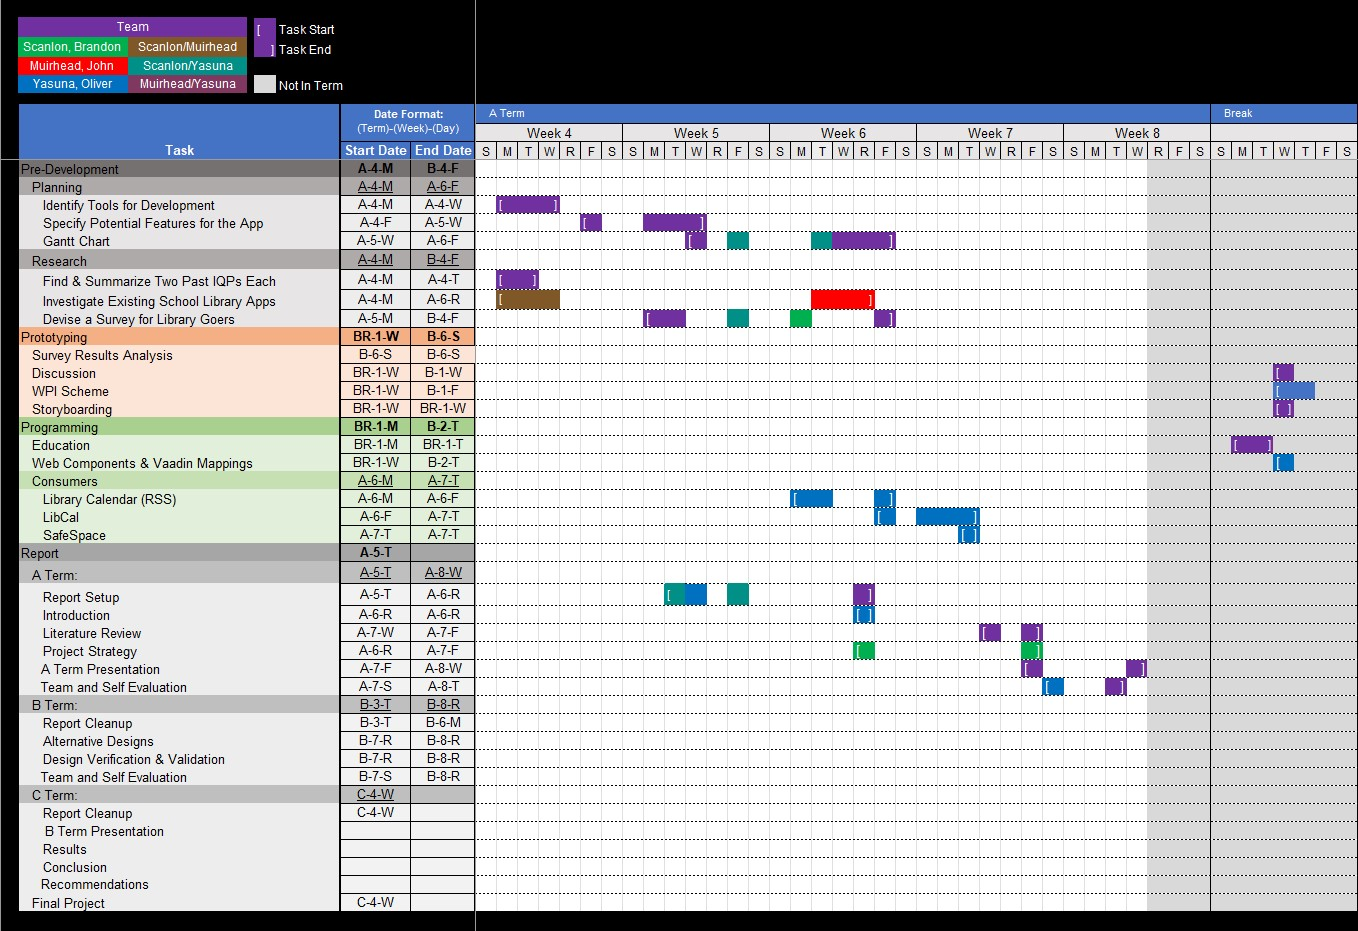
\includegraphics[scale=.58]{assets/img/Term A Timeline.jpg}
    \caption{Term A Project Timeline}
    \label{fig:project_timeline}
\end{figure}

\begin{figure}[H]
 \hspace*{-2.25cm}
    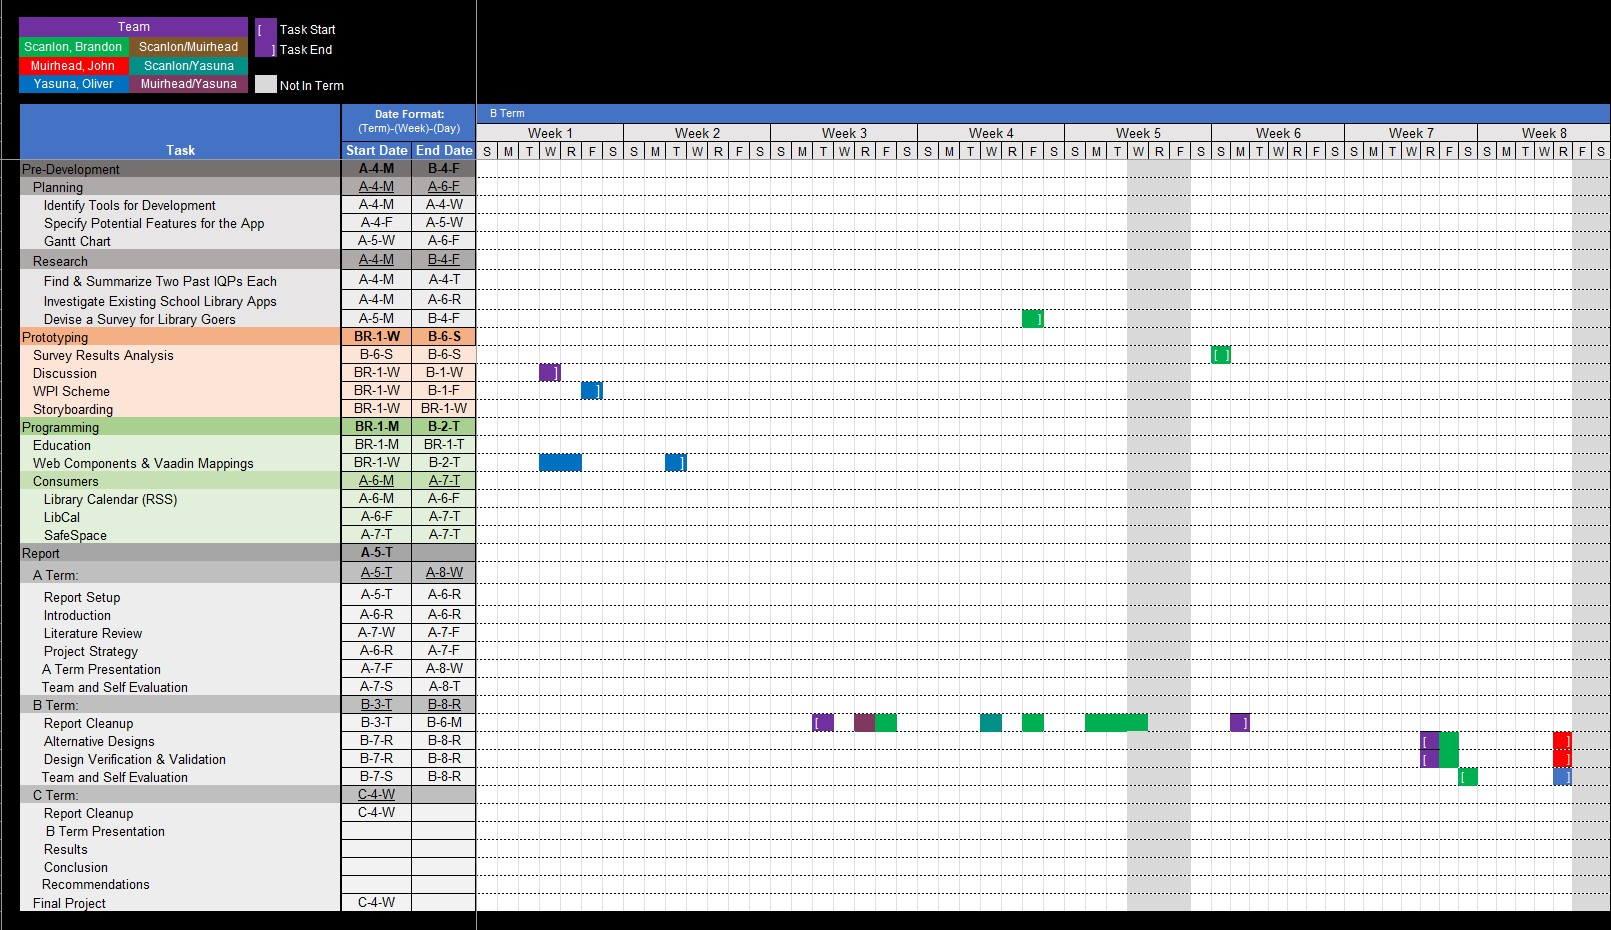
\includegraphics[scale=.49]{assets/img/Term B Timeline.jpg}
    \caption{Term B Project Timeline}
    \label{project_timeline}
\end{figure}
